\documentclass[a4paper,11pt,fleqn]{article}%fleqn pour aligner les equations à gauche
\usepackage{../../Styles/Cours}

\newcommand{\chnum}{Chapitre 3}
\newcommand{\chtitle}{Suivi cinétique d'une transformation chimique}
\newcommand{\dtype}{TP}

\begin{document}
\maketitle

Lors ce cette séance de TP, un suivi de la réaction entre les ions iodure \ce{I-(aq)} et les ions peroxodisulfates \ce{S2O8^2-(aq)} sera réalisé par spectrophotométrie.

\begin{figure}[h!]
    \begin{minipage}[t]{.5\textwidth}
        \caption*{\textbf{Document 1 : Loi de vitesse d'ordre 1}}
        Soit un réactif $X$ en solution aqueuse. La vitesse volumique $v_X$ de disparition de l'espèce $X$ est traduite par la relation : $$v_X(t)=k\cdot [X](t)$$
        où $k$ est appelée constante volumique de vitesse (en \unit{\per\second})\\
        Comme $v_X = -\dfrac{d[X]}{dt}$, la loi de vitesse d'ordre 1 aboutit à la relation : $$k\cdot [X] = \dfrac{-d[X]}{dt}$$
        Toutes les fonctions du temps vérifiant cette dernière égalité sont de la forme : $[X](t) = [X]_0 \cdot e^{-k\cdot t}$, c'est à dire des fonctions exponentielles décroissantes
        \begin{minipage}{\textwidth}
        \caption*{\textbf{Couples oxydants-réducteurs}}
        \ce{I2(aq)}/\ce{I-(aq)}\\
        \ce{S2O8^2-(aq)}/\ce{SO4^2-(aq)}
        \end{minipage}
    \end{minipage}
    \begin{minipage}[t]{.5\textwidth}
    \caption*{\textbf{Document 2 : Spectre d'absorption du diiode}}
    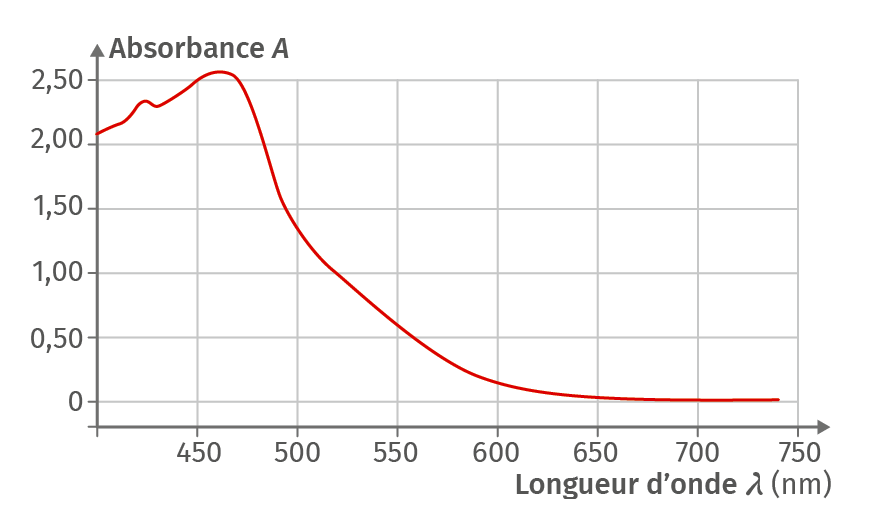
\includegraphics[width=\linewidth]{Ressources/TSPE_C10_AE2_Fig1.png}
    \end{minipage}
\end{figure}

\begin{enumerate}
    \item Écrire l'équation de la réaction étudiée.
    \item Observer le mélange réalisé au bureau. Préciser quelle espèce chimique est responsable de la coloration du milieu réactionnel.
    \item Justifier le choix de la spectrophotométrie comme technique de suivi cinétique.
    \item Déterminer, en justifiant, la longueur d'onde à laquelle régler le spectrophotomètre.
    \item Prévoir, en expliquant, l'allure de la courbe $A = f(t)$.
\end{enumerate}

\begin{center}\textbf{Appel n°1}\end{center}

\noindent \colorbox{gray!20}{\begin{minipage}{\linewidth}
    \textsc{À lire en entier avant de démarrer !}
    \begin{itemize}
        \item Paramétrer le spectrophotomètre en suivant les consignes de la fenêtre de dialogue et paramétrer l'acquisition temporelle en choisissant 500 points de mesure sur une durée de 30 minutes.
        \item Préparer, dans deux béchers distincts :
        \begin{itemize}
            \item un volume $V_1$ = \SI{10,0}{\milli\liter} d'une solution aqueuse d'iodure de potassium (\ce{K+} ; \ce{I-}) de concentration en soluté apporté $c_1$ = \SI{5,0E-1}{\mole\per\liter}
            \item un volume $V_2$ = \num{10,0} \unit{\milli\liter} d'une solution aqueuse de peroxodisulfate de sodium (\ce{2Na+} ; \ce{S2O8^2-}) en soluté apporté $c-2$ = \SI{8,0E-3}{\mole\per\liter}.
        \end{itemize}
        \item Mélanger les deux solutions préparées et \underline{lancer l'acquisition au moment du mélange}.
        \item Introduire \underline{le plus rapidement possible} un échantillon du mélange réactionnel précédent dans une cuve de spectrophotométrie
        \item Placer la cuve dans le spectrophotomètre.
    \end{itemize}
\end{minipage}}

\begin{center}\textbf{Appel n°2}\end{center}

\begin{enumerate}[resume]
    \item Déterminer le réactif limitant en complétant le tableau d'avancement. En déduire la concentration maximale en diiode $[\ce{I2}]_{max}$.
    \item Quelle semble être la valeur de l'absorbance maximale $A_{max}$ lorsque la réaction n'évolue plus ?
    \item A l'aide de la loi de Beer-Lambert et en admettant que la réaction est totale, déterminer l'expression de $[\ce{I2}]$, puis celle de $[\ce{S2O8^2-}]$ en fonction du temps.
    \item Modéliser la courbe donnant $[\ce{S2O8^2-}]$ en fonction du temps en faisant l'hypothèse d'une réaction d'ordre 1. Relever l'équation de la courbe.
    \item Déterminer $[\ce{S2O8^2-}]$ à $t=\SI{0}{s}$. Est ce en accord avec les données de l'énoncé ?
    \item Représenter la cette courbe et en déduire la constante volumique de vitesse $k$.
    \item Retrouver cette valeur dans la modélisation de la courbe donnant $[\ce{S2O8^2-}]$ en fonction du temps.
    \item Déterminer graphiquement le temps de demi-réaction $t_{1/2}$, c'est à dire la durée pour laquelle la concentration du réactif limitant a diminué de moitié.
\end{enumerate}
\begin{table}[h!]
    \centering
    \caption*{\textbf{Tableau d'avancement}}
    \begin{tabular}{|>{\centering}m{3cm}|m{3cm}|m{2cm}|m{2cm}||m{2cm}|m{2cm}|}\hline
        \multicolumn{2}{|>{\centering}m{6cm}|}{Équation de la réaction} & \multicolumn{4}{|m{8cm}|}{}\\
        \hline Etat du système & Avancement (en \unit{\mole}) & \multicolumn{4}{|m{8cm}|}{Quantités de matière (en \unit{\mole})}\\
        \hline Etat Initial & $x=0$ & $n_1 = $ & $n_2 =$ & &\\
        \hline En cours & $x$ & & & & \\
        \hline Etat final & $x_{max} =$ & & & & \\
        \hline
    \end{tabular}
    
    \label{tab:my_label}
\end{table}
\end{document}